\chapter{Grundlagen}
\label{sec:grundlagen}


\section{Software-Qualität}
\label{sec:softwarequalität}

Nahezu jeder Programmierer ist schon einmal mit dem Begriff der Software-Qualität in Berührung gekommen. Diesen Qualitätsbegriff jedoch genau zu fassen erweist sich als schwierig.
Die DIN-ISO-Norm 9126 definiert Software-Qualität wie folgt:
\\
\glqq Software-Qualität ist die Gesamtheit der Merkmale und Merkmalswerte eines Software-Produkts, die sich auf dessen Eignung beziehen, festgelegte Erforderniss zu erfüllen.\grqq \cite{iso/iec_iso/iec_2001}
\\
Aus dieser Definition wird deutlich, dass es sich bei dem Begriff der Software-Qualität eine multikausale Größe handelt. Das bedeutet, dass zur Bestimmung der Qualität einer Software nicht ein einzelnes Kriterium existiert. Vielmehr verbergen sich hinter dem Begriff eine ganze Reihe verschiedener Kriterien die je nach den gestellten Anforderungen in ihrer Relevanz variieren.\cite[vgl. Seite 6 ff.]{hoffmann_software-qualitat_2013}
Sammlungen solcher Kriterien werden in sogenannten Qualitätsmodellen zusammengefasst. Die DIN-ISO-Norm 9126 bietet selbst ein solches Qualitätsmodell und definiert damit eine Reihe von wesentlichen Merkmalen, die für die Beurteilung der Software-Qualität eine Rolle spielen. Diese Merkmale sind in der Abbildung \ref{fig:qualitaetsmerkmaleVonSoftwaresystemen} zusammengefasst.
\begin{figure}[htb]
  \centering  
  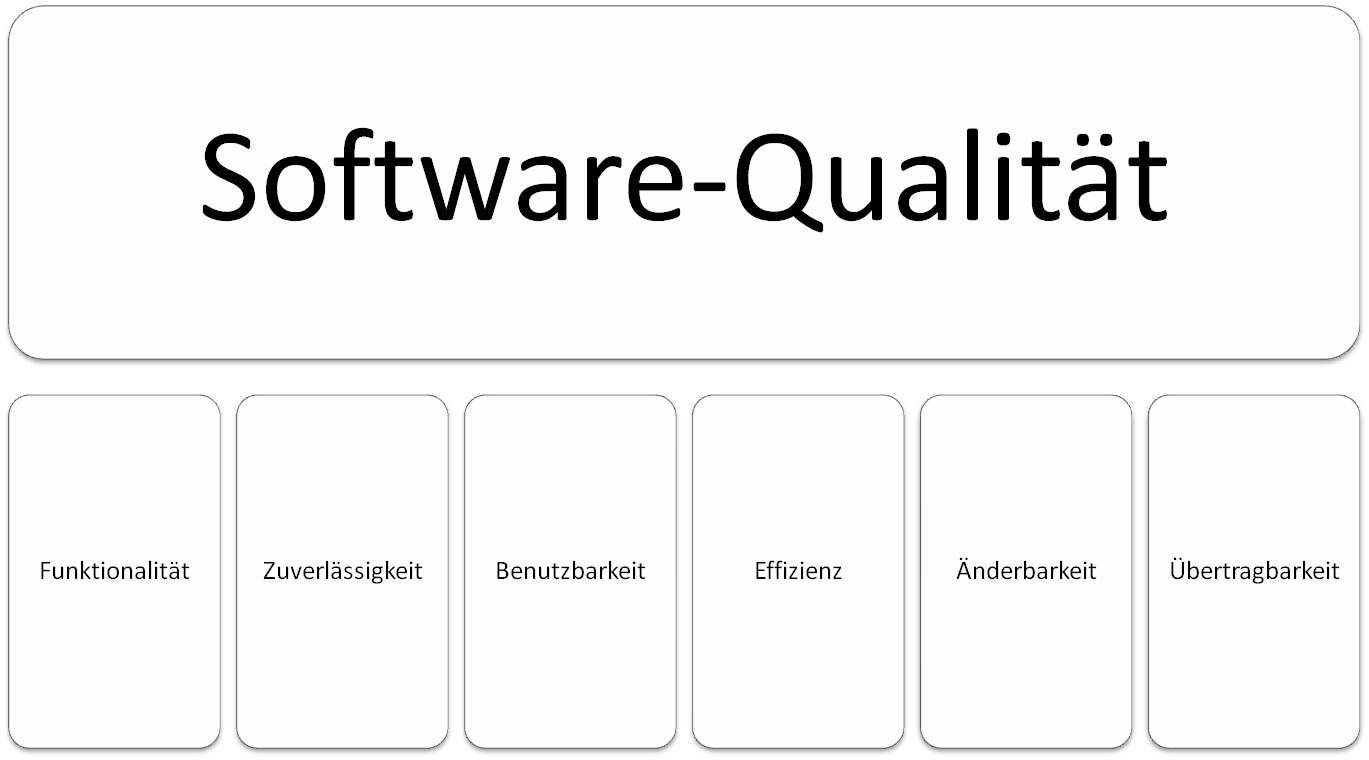
\includegraphics[scale=0.6]{img/softwarequalitaet9126.png}\\
  \footnotesize\sffamily\textbf{Quelle:} \cite{iso/iec_iso/iec_2001}
  \caption{Qualitätsmerkmale von Softwaresystemen (ISO 9126)}
  \label{fig:qualitaetsmerkmaleVonSoftwaresystemen}
\end{figure}
Eine nähere Definition der einzelnen Begriffe des Qualitätsmodells kann beispielsweise dem Buch Software-Qualität von Dirk W. Hoffmann entnommen werden. \cite[Seite 7 ff.]{hoffmann_software-qualitat_2013}
Um die Qualität einer Software zu Steigern, bietet die moderne Software-Qualitätssicherung eine Vielzahl von Methoden und Techniken.
Ein Teil der Methoden geht dabei davon
aus, dass ein qualitativ hochwertiger Prozess der Produkterstellung die Entstehung von qualitativ hochwertigen Produkten begünstigt. Das Augenmerk wird hierbei also auf die Prozessqualität gelegt. Diese Methoden fallen in den Bereich der Prozessqualität.
Die klassischen Vorgehensmodelle der Softwarentwicklung
werden z.B. hier eingeordnet. Einen weiteren Bereich bilden die Methoden die zur Verbesserung der  Produktqualität dienen. Bei diesen Methoden wird das Softwareprodukt direkt bezüglich der Qualitätsmerkmale überprüft. Dieser Bereich unterteilt sich in die konstruktiven und analytischen Qualitätssicherung. Unter konstruktiver Qualitätssicherung versteht man den Einsatz von z.B. Methoden, Werkzeugen oder Standards die
dafür sorgen, dass ein Produkt bestimmte Forderungen erfüllt. 
Unter analytische Qualitätssicherung versteht man den Einsatz von analysierenden bzw. prüfenden Verfahren, die Aussagen
über die Qualität eines Produkts machen.
In diesem Bereich der Qualitätssicherung befindet sich beispielsweise der klassische Software-Test.\cite[vgl. Seite 19 ff.]{hoffmann_software-qualitat_2013} Eine Übersicht über das gesamte Gebiet der SoftwareQualitätssicherung, wie es sich uns gegenwärtig darstellt, ist in Abbildung \ref{fig:softwareQualitätssicherung} dargestellt. 
\begin{figure}[htb]
  \centering  
  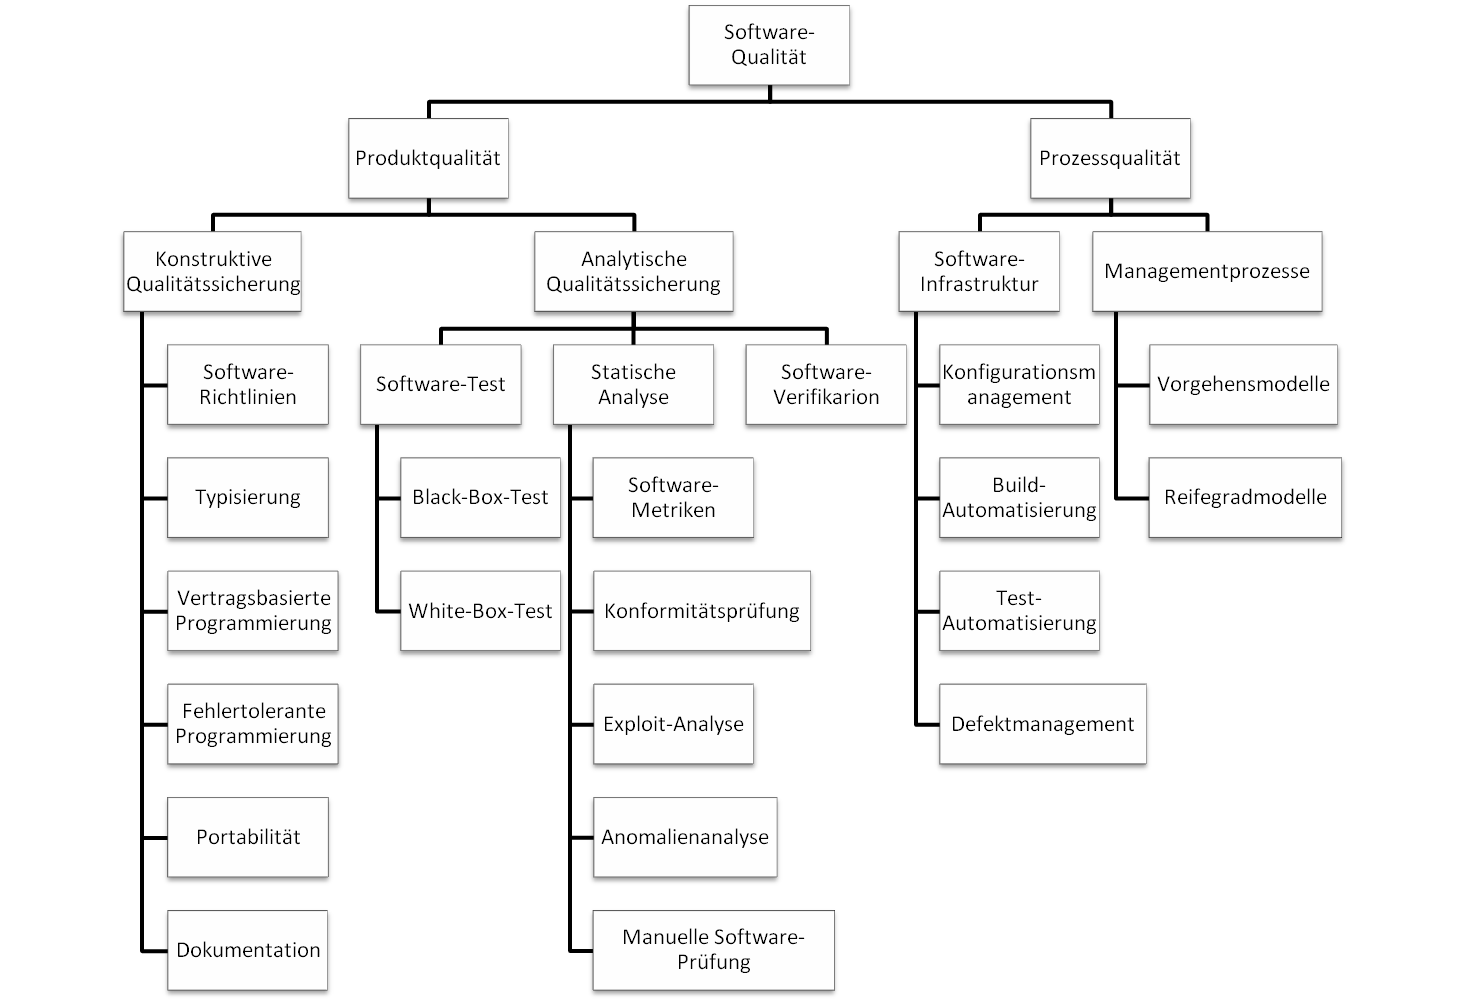
\includegraphics[scale=0.7]{img/softwarequalitaet.png}\\
  \footnotesize\sffamily\textbf{Quelle:} \cite[vgl. Seite 20]{hoffmann_software-qualitat_2013}
  \caption{Übersicht über das Gebiet der Software-Qualitätssicherung}
  \label{fig:softwareQualitätssicherung}
\end{figure}



\section{Softwaretest}
\label{sec:softwaretest}
Im laufe der Zeit wurden viele Versuche unternommen um die Qualität von Software zu steigern. Besondere Bedeutung hat dabei der Software-Test erlangt.
Der IEEE Std 610.12 definiert den Begriff Test als das ausführen einer Software unter bestimmten Bedingungen mit dem Ziel, die erhaltenen Ergebnisse auszuwerten, also gegen erwartete Werte zu vergleichen.
(Im Original: \glqq An activity in which a system or component is executed under specific conditions, the results are observed or recorded, and an evaluation is made of some aspect of the system or component.\grqq\ \cite{ieee_ieee_1991})
Bereits zu beginn der Softwareentwicklung hat man versucht Programme vor ihrer Auslieferung zu testen. Der dabei erzielte Erfolg entsprach nicht immer den Erwartungen. Im laufe der Jahre wurde das Testen daher auf eine immer breitere Grundlage gestellt. Es entwickelten sich Unterteilungen des Software-Tests die bis heute bestand haben. Hier wären zu nennen:
\begin{itemize}
\item White-Box-Test
\item Black-Box-Test und externe Testgruppe
\item Volume Test, Stress Test und Test auf Systemebene
\end{itemize}
Jeder dieser Begriffe beschreibt bestimmte Techniken, die bei konsequenter Anwendung dazu führen können Fehler in Softwareprodukten zu identifizieren. \cite[vgl. Seite 18]{thaller_software-test_2002}

Neben der Auswahl der richtigen Techniken für ein bestimmtes Problem spielt in der Praxis die Testkonstruktion eine zentrale Rolle. Bereits für kleine Programme ist es faktisch nicht mehr möglich das Verhalten einer Software für alle möglichen Eingaben zu überprüfen. Es muss sich daher immer auf eine vergleichsweise winzige Auswahl an Testfällen beschränkt werden. Testfälle unterscheiden sich jedoch stark in ihrer Relevanz. Die Auswahl der Testfälle hat daher einen großen Einfluss auf die Anzahl der gefundenen Fahler und damit auch auf die Qualität des Endprodukts. \cite[vgl. Seite 22]{hoffmann_software-qualitat_2013}

Dennoch ist der Software-Test eines der am meisten verbreiteten Techniken zur Verbesserung der Softwarequalität. Diese Technik alleine reicht jedoch nicht aus um über lange Sicht gute Software zu produzieren. Ein großer Nachteil des Softwaretests ist es, dass Fehler erst in einer relativ späten Phase der Entwicklung identifiziert werden. Je später eine Fehler jedoch entdeckt wird, umso teurer wird auch seine Beseitigung. Abbildung \ref{fig:softwareQualitätssicherung} zeigt, dass der Software-Test nur eine von vielen Techniken des Qualitätsmanagement darstellt. Um die Probleme des Software-Tests auszugleichen, ist es daher ratsam, sich bei der Qualitätssicherung möglichst breit aufzustellen und sich nicht nur auf die analytische Qualitätssicherung in Form des Software-Tests zu verlassen. \cite[vgl. Seite 18]{thaller_software-test_2002}


\section{Testautomatisierung}
\label{sec:testautoGrundlagen}
Das Testen von Software macht in heutigen Projekten einen großen Teil der Projektkosten aus. Studien haben gezeigt, dass das Testen für 50\% 
und mehr der gesamten Projektkosten verantwortlich sein kann. \cite{ramler_economic_2006}
Mit Steigender Komplexität der Softwäre steigen diese Kosten immer weiter an.
Um diese Kosten zu reduzieren haben sich im laufe der Zeit die bestehenden Testmethoden immer weiter entwickelt und auch neue Ansätze herausgebildet. Einer dieser Ansätze ist es Software-Tests möglichst automatisiert durchzuführen. Diesen Ansatz fast man mit dem Begriff Testautomatisierung zusammen.
Seidl et al. definieren Testautomatisierung als \glqq die Durchführung von ansonsten manuellen Testtätigkeiten durch Automaten.\grqq \cite[Seite 7]{seidl_basiswissen_2012}
Diese Definition zeigt, dass das Spektrum der Testautomatisierung breit gefächert ist. Testautomatisierung beschränkt sich nicht nur auf das automatisierte durchführen von Testfällen sondern erstreckt sich über alle Bereiche des Software-Test. [ KAPITEL ... BEFASST SICH NÄHER MIT DEN VERSCHIEDENEN BEREICHEN UND ANSÄTZEN DER TESTAUTOMATISIERUNG].
Aus Sicht des Qualitätsmanagement ist die Testautomatisierung sowohl den Methoden zur Steigerung der Produktqualität als auch der Prozessqualität zugeordnet. Ein automatisierter Software-Test hat immer noch den selben Charakter wie ein manueller Software-Test und ist daher ein Teil der analytischen Qualitätssicherung. Allerdings erfordert Testautomatisierung auch immer infrastrukturelle Anpassungen. Automatisierte Testfälle benötigen in der Regel eine Besondere Software-Infrastruktur wie etwa ein Automatisierungsframework. Solche Maßnahmen, die den Programmentwickler aus technischer Sicht in die Lage versetzen, seiner täglichen Arbeit in geregelter und vor allem produktiver Weise nachzugehen, werden den Methoden zur Verbesserung der Prozessqualität zugeordnet. (siehe Abbildung \ref{fig:softwareQualitätssicherung}).
\cite[vgl. Seite 25]{hoffmann_software-qualitat_2013}


\section{Testprozess}
\label{sec:testprozess}

Um Software-Tests effektiv und Strukturiert durchzuführen wird eine verfeinerter Ablaufplan für die einzelnen Testaufgaben benötigt. Diesen Ablaufplan fassen Splinner und Linz im fundamentalen Testprozess zusammen. Die einzelnen Arbeitsschritte die im Lebenszyklus eines Software-Tests anfallen werden dabei verschiedenen Phasen zugeordnet.
Durch den Testprozess wird die Aufgabe des Testens so in kleinere Testaufgaben untergliedert.

Testaufgaben, die man dabei unterscheidet sind:

\begin{itemize}
	  \itemsep0pt
      \item Testplanung und Steuerung
      \item Testanalyse und Testdesign
      \item Testrealisierung und Testdurchführung
      \item Testauswertung und Bericht
      \item Abschluss der Testaktivitäten       
\end{itemize}

Obgleich die Aufgaben in sequenzieller Reihenfolge im Testprozess angegeben sind, können sie sich überschneiden und teilweise auch gleichzeitig durchgeführt werden. Auf Grundlage des fundamentalen Testprozesses nach Splinner und Linz werden im folgenden diese Teilaufgaben näher beschrieben. \cite[S.20ff]{spillner_basiswissen_2007}

\subsection{Testplanung und Steuerung}
\label{subsec:testplanung_und_steuerung}


\subsection{Testanalyse und Testdesign}
\label{subsec:testanalyse_und_design}


\subsection{Testrealisierung und Testdurchführung}
\label{subsec:testrealisierung_und_durchführung}

\subsection{Testauswertung und Bericht}
\label{subsec:testauswertung_und_bericht}


\subsection{Abschluss der Testaktivitäten}
\label{subsec:abschluss_der_testaktivitäten}



\section{Softwarelebenszyklus}
\label{sec:softwarelebenszyklus}



\subsection{V-Modell}
\label{subsec:vmodell}
\subsection{Agil}
\label{subsec:agil}

